\chapter{Projekt: offline grafický editor}
\label{sect:editor}

Majme dvojrozmerné pole \vb{obr} s $r$ riadkami a $s$ stĺpcami. Bod v rovine
so súradnicami $x,y$ (kde $x$, $y$ sú reálne čísla) sa zobrazí na pixel
\prg!obr[r-(int)y][(int)x]!:\\


\centerline{
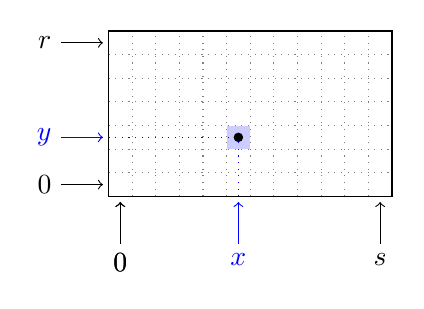
\begin{tikzpicture}[scale=0.3]
  \def\X{12}
  \def\Y{7}
  \def\x{5}
  \def\y{3}
  \filldraw[draw=none,fill=blue!20!white](\x,\y-1) rectangle (\x+1,\y);
  \filldraw[fill=black](\x+0.5,\y-0.5) circle (5pt);
  \draw[thin,gray,dotted](0,0) grid (\X,\Y);
  \draw(0,0) rectangle (\X,\Y);
  \draw[->, shorten >= 2] (0.5,-2) node[anchor=north]{0} -- (0.5,0);
  \draw[->, shorten >= 2] (\X-0.5,-2) node[anchor=north]{$s$} -- (\X-0.5,0);
  \draw[->, shorten >= 2] (-2,0.5) node[anchor=east]{0} -- (0,0.5);
  \draw[->, shorten >= 2] (-2,\Y-0.5) node[anchor=east]{$r$} -- (0,\Y-0.5);
  \draw[->, shorten >= 2] (0.5,-2) node[anchor=north]{0} -- (0.5,0);
  
  \draw[blue,->, shorten >= 2] (\x+0.5,-2) node[anchor=north]{$x$} -- (\x+0.5,0);
  \draw[blue,->, shorten >= 2] (-2,\y-0.5) node[anchor=east]{$y$} -- (0,\y-0.5);
  \draw[thin,blue,dotted] (\x+0.5,0) -- (\x+0.5,\y-0.5) (0,\y-0.5) -- (\x+0.5,\y-0.5);

\end{tikzpicture}
}


Majme teraz nasledovnú úlohu. Máme dané dva body $A=[x_1,y_1]$, $B=[x_2,y_2]$
a chceme vykresliť čiaru z bodu $A$ do bodu $B$.
Ak čiara ide zvislo alebo vodorovne, 
 situácia je jednoduchá, stačí nám jeden cyklus. V opačnom 
 prípade máme viac roboty. 
Zober si priamku, ktorá prechádza bodmi $A$, $B$.
Keď sa z bodu $A$ presunieš do bodu $B$, prejdeš vo vodorovnom smere $x_2-x_1$
a vo zvislom smere $y_2-y_1$. Ak prejdeš do polovice cesty, dostaneš sa 
do bodu $X$:\\


\centerline{
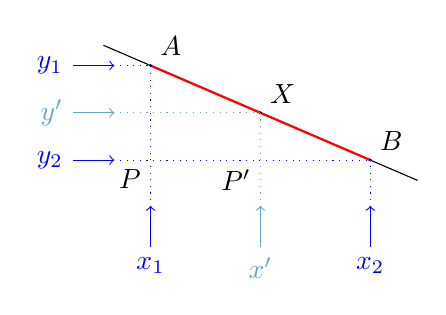
\begin{tikzpicture}[scale=0.3]
  \def\X{12}
  \def\Y{7}

  \def\x{1.3}
  \def\y{5.7}
  \def\ix{1}
  \def\iy{5}
  
  \def\xx{10.6}
  \def\yy{1.7}
  \def\ixx{10}
  \def\iyy{1}

  \pgfmathsetmacro{\s}{(\yy-\y)/(\xx-\x)}
  \pgfmathsetmacro{\dx}{\ix+0.5-\x}

  \def\ab {\x/\y,\xx/\yy}
  
  \pgfmathtruncatemacro{\n}{\ixx-\ix}
  

  \draw[thin] (\x-2,\y-2*\s)  -- (\xx+2,\yy+2*\s);
  \draw[thick,red] (\x,\y) -- (\xx,\yy);

  \foreach \a/\b[count=\i] in \ab {
  \filldraw[fill=black](\a,\b) circle (1pt);
  \draw[thin,blue,dotted] (\a,0) -- (\a,\b) (0,\b) -- (\a,\b);
  \draw[blue,->, shorten >= 2] (\a,-2) node[anchor=north]{$x_\i$} -- (\a,0);
  \draw[blue,->, shorten >= 2] (-2,\b) node[anchor=east]{$y_\i$} -- (0,\b);
  }
  
  \pgfmathsetmacro{\a}{\x+0.5*(\xx-\x)}
  \pgfmathsetmacro{\b}{\y+\s*0.5*(\xx-\x)}
  \filldraw[fill=black](\a,\b) circle (1pt);
  \def\tmp{cyan!50!gray}
  \draw[thin,draw=\tmp,dotted] (\a,0) -- (\a,\b) (0,\b) -- (\a,\b);
  \draw[\tmp,->, shorten >= 2] (\a,-2) node[anchor=north]{$x'$} -- (\a,0);
  \draw[\tmp,->, shorten >= 2] (-2,\b) node[anchor=east]{$y'$} -- (0,\b);

  \node[anchor = south west] at(\x,\y) {$A$};
  \node[anchor = south west] at(\xx,\yy) {$B$};
  \node[anchor = south west] at(\a,\b) {$X$};
  \node[anchor = north east] at(\a,\yy) {$P'$};
  \node[anchor = north east] at(\x,\yy) {$P$};



\end{tikzpicture}
}

Pretože $\triangle APB$ a $\triangle XP'B$ sú podobné, tak pri ceste do bodu $X$
prejdeš polovičnú vzdialenosť vo vodorovnom smere, aj polovičnú vzdialenosť v 
zvislom smere, t.j. v smere osi $x$ sa posunieš o $0.5(x_2-x_1)$ a v smere osi 
$y$ o $0.5(y_2-y_1)$. Toto platí všeobecne: ak sa na osi $x$ posunieš o 
$c(x_2-x_1)$, na osi $y$ sa posunieš o $c(y_2-y_1)$. 
Ak si za $c$ zoberiem $\frac{1}{x_2-x_1}$, tak 
 keď som v nejakom bode na priamke
 a v smere osi $x$ sa pohnem o $c(x_2-x_1)=1$, tak v smere osi $y$ sa pohnem o 
 $c(y_2-y_1)=\frac{y_2-y_1}{x_2-x_1}$. \indexItem{Mat}{sklon priamky} Číslo $s=\frac{y_2-y_1}{x_2-x_1}$ budem 
 volať {\em sklon} priamky: ak sa v smere $x$ pohnem na priamke o $1$,
 v smere $y$ sa pohnem o $s$.
 Predpokladajme, že $x_1<x_2$ a $-1\le s\le1$,
 t.j. ak sa pohnem o 1 v smere osi $x$, v smere osi $y$ sa pohnem o menej ako 1.
 

\vskip 2ex
\centerline{
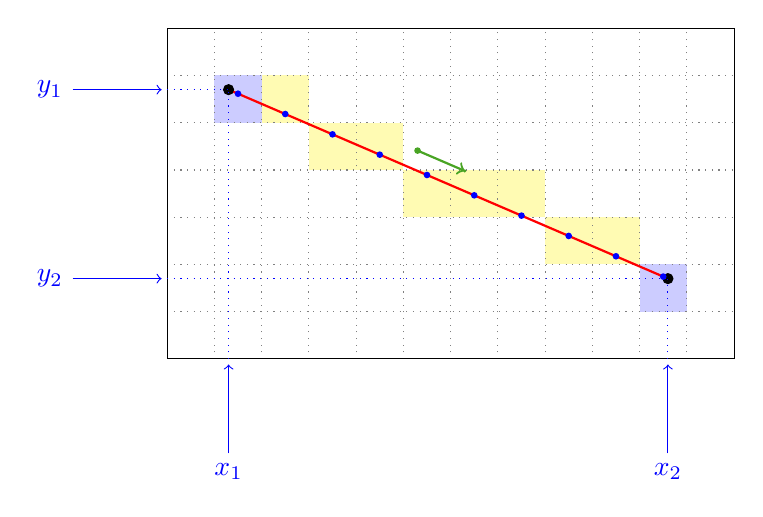
\begin{tikzpicture}[scale=0.6]
  \def\X{12}
  \def\Y{7}

  \def\x{1.3}
  \def\y{5.7}
  \def\ix{1}
  \def\iy{5}
  
  \def\xx{10.6}
  \def\yy{1.7}
  \def\ixx{10}
  \def\iyy{1}

  \pgfmathsetmacro{\s}{(\yy-\y)/(\xx-\x)}
  \pgfmathsetmacro{\dx}{\ix+0.5-\x}

  \def\ab {\x/\y/\ix/\iy,\xx/\yy/\ixx/\iyy}
  
  \pgfmathtruncatemacro{\n}{\ixx-\ix}
  
  \foreach \i in {0,...,\n} {
    \pgfmathtruncatemacro{\tmpx}{\ix+0.5+\i}
    \pgfmathtruncatemacro{\tmpy}{\y+(\dx+\i)*\s}
    \filldraw[draw=none,fill=yellow!30!white] (\tmpx,\tmpy) rectangle 
    (\tmpx+1,\tmpy+1);
.
  }
  
  \foreach \a/\b/\ia/\ib[count=\i] in \ab {
  \filldraw[draw=none,fill=blue!20!white](\ia,\ib) rectangle (\ia+1,\ib+1);
  }

  \draw[thin,gray,dotted](0,0) grid (\X,\Y);
  \draw(0,0) rectangle (\X,\Y);
  \draw[thick,red] (\x,\y) -- (\xx,\yy);

  \foreach \a/\b/\ia/\ib[count=\i] in \ab {
  \filldraw[fill=black](\a,\b) circle (3pt);
  \draw[thin,blue,dotted] (\a,0) -- (\a,\b) (0,\b) -- (\a,\b);
  \draw[blue,->, shorten >= 2] (\a,-2) node[anchor=north]{$x_\i$} -- (\a,0);
  \draw[blue,->, shorten >= 2] (-2,\b) node[anchor=east]{$y_\i$} -- (0,\b);
  }

  \def\rst{rgb:green,5;yellow,4;blue,2;black,3}

  \filldraw[draw=none,fill=\rst] (\x+4,\y+3*\s) circle (2pt)
  (\x+5,\y+4*\s) circle (1pt);
  \draw[->,draw=\rst, thick] (\x+4,\y+3*\s) -- (\x+5,\y+4*\s);

  \foreach \i in {0,...,\n} {
    \pgfmathsetmacro{\tmp}{\y+(\dx+\i)*\s}
    \filldraw[draw=none,fill=blue] (\ix+0.5+\i,\tmp) circle (2pt);

  }

\end{tikzpicture}
}


Na nakreslenie čiary stačí vyrátať $s$, pohnúť sa na priamke tak, aby 
som bol v smere $x$-ovej osi v strede počiatočného pixelu
(prvá modrá bodka, súradnice\footnote{\indexItem{Mat}{dolná celá časť}%
  v matematike sa zvykne písať $\lfloor x\rfloor$ na označenie dolnej
celej časti, t.j. najbližšieho menšieho celého čísla. Treba dať pozor na to, že
$\lfloor x\rfloor=$\prg!(int)x! iba pre kladné čísla, napr. \prg!(int)3.14 == 3!.
Pre záporné čísla to ale neplatí: $\lfloor-3.14\rfloor=-4$, ale \prg!(int)(-3.14)==-3!.} $\lfloor x_1\rfloor+0.5$ a 
 \hbox{$y_1+s(\lfloor x_1\rfloor+0.5-x_1)$}) a potom
postupne sa vždy pohnúť o 1 v smere osi $x$ a o $s$ v smere osi $y$ a zafarbiť
príslušný pixel (na obrázku žlté).


Ak by naopak $s<-1$ alebo $s>1$, to znamená, že ak sa pohnem o 1 v smere osi $x$,
v smere osi $y$ sa môžem pohnúť o veľa. Preto keby som použil tento istý program,
môže sa mi stať, že niektoré pixely preskočím. Preto to treba urobiť naopak:
posunúť sa vždy o 1 v smere osi $y$ a dorátať si pozíciu v smere osi $x$.
Skús si to premyslieť a naprogramovať.

\begin{uloha}
  \label{uloha:editor}
  Napíš program, ktorý prečíta postupnosť príkazov (na každom riadku jeden)
  a podľa nich vyrobí obrázok.
  Príkazy môžu byť
\def\tmp{\item \textcolor{magenta}}  
\begin{itemize}\itemsep=-1mm
    \tmp{\vb{i} {\em sirka vyska}} 
      (init) Toto je vždy prvý príkaz (a je v zozname iba
      raz). Nastaví rozmery obrázka. 
      \tmp{\vb{c} r g b} (color) Nastaví farbu na $\{r,g,b,255\}$.
    \tmp{\vb{m} x y} (move) Presunie sa do bodu $[x,y]$ (bez kreslenia).
    \tmp{\vb{l} x y} (line) Nakreslí čiaru (aktuálnou farbou) 
    z aktuálneho bodu do bodu $[x,y]$.
    \tmp{\vb{f} x y r g b} (fill) Vyplní aktuálnou farbou oblasť, ktorej okraje
    sú ohraničené pixelmi buď aktuálnej farby alebo farby $\{r,g,b,255\}$ 
    (spomeň si na úlohu~\ref{uloha:fill})
    \tmp{\vb{s} meno} (save) Uloží obrázok a skončí.
\end{itemize}

Napríklad tento vstup vyrobí obrázok vpravo

  \begin{column}{0.45}
\begin{Verbatim}
i 800 600
m 50 300
l 220 100
l 700 450
l 700 150
l 220 500
l 50 300
c 150 255 30
f 220 220 0 0 0
f 650 300 0 0 0
c 255 0 0
m 120 350
l 150 380
l 180 350
l 150 320
l 120 350
c 255 255 255
f 130 340 255 0 0
s edit.png
\end{Verbatim}
  \end{column}\hfill\begin{column}{0.45}
  {
\setlength{\fboxsep}{0pt}
\fbox{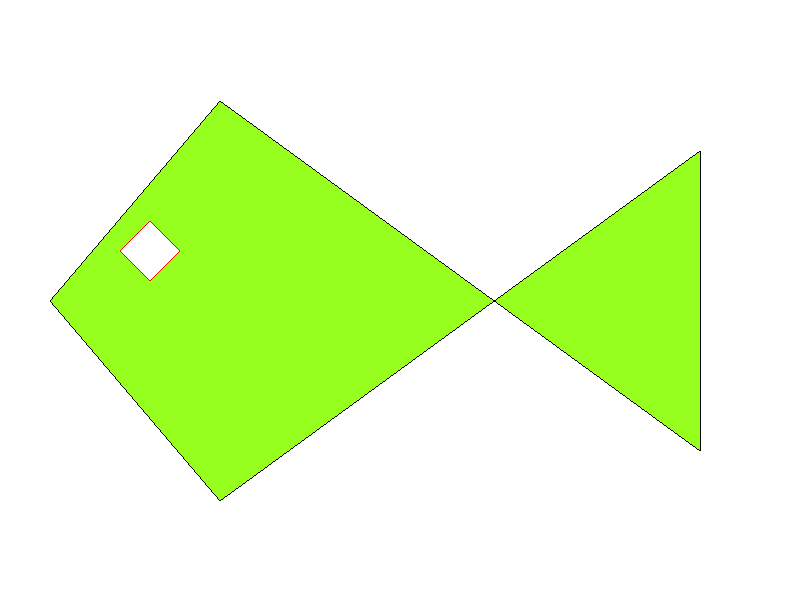
\includegraphics[width=\textwidth]{data/edit.png}}
  }
\end{column}
  \end{uloha}

  \begin{column}{0.65}
\begin{uloha}
  Uvažujme nasledovnú variáciu na tému Sierpińského koberca: máme parametre
  \prg!int x!, \prg!int d!,
  \prg!double i! a \prg!double f!. Chceme mať vzorku na obrázku rozmerov $x\times x$.
  Vzorka stupňa $d$  je štvorec so stranou dĺžky $ix$ umiestnený v strede obrázka.
  Navyše, ak $d>1$ tak v každom z rohov štvorca umiestnime vzorku stupňa $d-1$
  zmenšenú o faktor $f$ (a môže mať upravenú farbu). Napríklad pre
  hodnoty \vb{1000 6 0.45 0.5} by vzorka mohla vyzerať ako na obrázku vpravo.
  
  Napíš program, ktorý načíta zo vstupu parametre \vb{x d i f} a vypíše postupnosť príkazov,
  na základe ktorej program z predchádzajúcej úlohy vykreslí 
  vzorku.
\end{uloha}
\end{column}\hfill\begin{column}{0.3}
  {\setlength{\fboxsep}{0pt}
  \centerline{\fbox{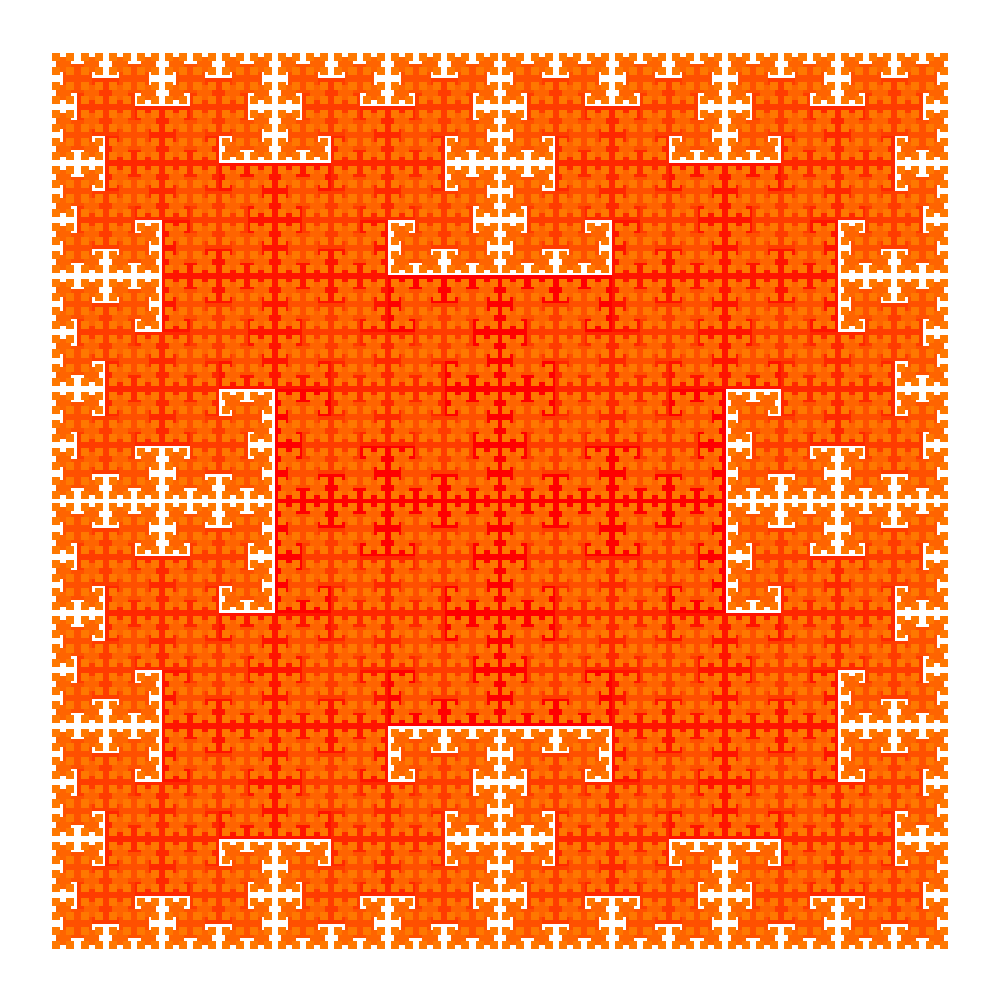
\includegraphics[width=\textwidth]{data/qq.png}}}
  }
\end{column}  


\indexItem{Mat}{sin, cos}
\section*{Odbočka: goniometrické funkcie $\sin$ a $\cos$}
\label{sect:sin_cos}

Niekedy je dobré vedieť kresliť čiaru nie do konkrétneho bodu, ale pod istým uhlom.
Povedzme, že máme uhol $\alpha$ okolo bodu $P$. Urobíme si hocikoľko
kolmíc takto:\\


\centerline{
  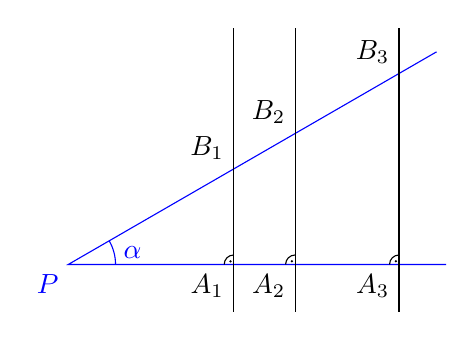
\begin{tikzpicture}[scale=0.6]
  \def\an{30}
  \def\len{8}
  \def\ra{0.2}
  \draw[blue](\len,0) -- (0,0) node[anchor=north east]{$P$} -- (\an:\len+1);
  \draw[blue](1,0) arc (0:\an:1) node[midway,anchor=west]{$\alpha$};

  \foreach \x[count=\i] in {3.5,4.8,7} {
    \draw(\x,-1) -- (\x,5);
    \node[anchor=north east] at (intersection of 0,0--10,0 and \x,-1--\x,5) {$A_{\i}$};
    \node[anchor=south east] at (intersection of 0,0--\an:100 and \x,-1--\x,5) {$B_{\i}$};
    \draw (\x,\ra) arc (90:180:\ra);
    \filldraw (\x-\ra/3,\ra/3) circle (.3pt);
  }
\end{tikzpicture}}


Všetky trojuholníky $\triangle A_1PB_1$,  $\triangle A_2PB_2$, \ldots sú podobné: majú
všetky uhly rovnako veľké. Preto sa zachovávajú aj pomery strán: napr.\footnote{%
  znakom $\nrm{\cdot}$ označujem dĺžku
}
$\nrm{A_3P} = 2\nrm{A_1P}$, preto aj $\nrm{B_3P}=2\nrm{B_1P}$. To znamená, že 
$\frac{\nrm{A_3P}}{\nrm{B_3P}}=\frac{2\nrm{A_1P}}{2\nrm{B_1P}}=\frac{\nrm{A_1P}}{\nrm{B_1P}}$.
Inými slovami, pomer $\frac{\nrm{A_iP}}{\nrm{B_iP}}$ je stále rovnaký, nezáleží, ktorú kolmicu
$A_iB_i$ si zoberieme. Tento pomer závisí iba od uhla $\alpha$, a označuje sa $\cos(\alpha)$
({\em kosínus}). Podobne pomer $\frac{\nrm{B_iA_i}}{\nrm{B_iP}}$ závisí iba od $\alpha$
a označuje sa $\sin(\alpha)$ ({\em sínus}).


Na čo je dobré poznať hodnoty $\sin(\cdot)$ a $\cos(\cdot)$? Povedzme, že chceš zistiť,
aké súradnice má bod $B$, ktorý je od $[0,0]$ vo vzdialenosti $r$ pod uhlom $\alpha$:


\centerline{
  \begin{tikzpicture}[scale=3.5]
  \def\an{40}
  \def\ra{0.4ex}
    \draw[thin,dotted,step=0.5](-0.5,-0.5) grid (1,1);
    \draw(1.1,0) -- (0,0) node[anchor=north east]{$O=[0,0]$} -- (\an:1.1);

    \draw[red](1ex,0) arc (0:\an:1ex) node[midway,anchor=west]{$\alpha$};
    \draw[thin,gray](-35:1) arc (-35:125:1);

    \draw[-{>[length=3ex,width=1ex]},thin,gray] (0,0) -- (110:1) node[midway,anchor=east]
    {$r$};

    \coordinate (B) at (\an:1);
    \draw[red](0,0)--(B) node[midway,anchor=south east]{$r$};
    \node[right=3mm of B]  {$B=[x,y]$};

    \draw[blue] (B) -- (B|-0,0) coordinate (A) node[midway, anchor=west] {$y = r\sin(\alpha)$};
    \node[anchor=north west] at (A) {$A$};
    
    \draw (A)+(0,\ra) arc (90:180:\ra);
    \filldraw (A)+(-\ra/3,\ra/3) circle (.1pt);

    \def\g{rgb:green,5;yellow,4;blue,2;black,3}
    \draw[thick,draw=\g](0,0)--(A) 
    node[midway,anchor=north]{\textcolor{\g}{$x = r\cos(\alpha)$}};
\end{tikzpicture}}


Keď si z $B$ spravíš kolmicu, dostaneš pravouhlý $\triangle AOB$, pričom $\nrm{OA}=x$,
$\nrm{AB}=y$ sú hľadané súradnice bodu $B$. Z predchádzajúceho vieš, že 
$\cos(\alpha)=\frac{\nrm{OA}}{\nrm{OB}}=\frac{x}{r}$, preto $x=r\cos(\alpha)$.
Rovnako dostaneš $y=r\sin(\alpha)$.


\indexItem{Prg}{\vb{cmath}}Funkcie \prg!sin! a \prg!cos! sú prístupné v knižnici, ktorá sa volá \vb{cmath}. 
Ich vstup ale nie je v stupňoch, ale v {\em radiánoch}. Ak obsah kruhu\footnote{%
  Urob si takýto pokus: zober si riešenie úlohy~\ref{uloha:kruh}
  a zrátaj v premennej \vb{S} počet čiernych pixelov. Na konci programu vypíš
  pomer čiernych pixelov k obsahu štvorca so stranou $r$, t.j. 
  \prg!(double)S / (double)(r * r)! Pre $r=10$ bol môj výsledok $3.05$, pre
  $r=500$ to už bolo $3.14128$ a pre $r=2450$ to bolo $3.14157$.

  
\begin{tikzpicture}
\begin{axis}[
  % title={\vb{pi}},  
  width=\textwidth, 
  height=4cm,
  xlabel={$r$},
  scaled x ticks=false,
  scaled y ticks=false,
  domain=0:800,
  xmin=0,
  xmax=800,
  ymin=3.05,
  ymax=3.15,
  /pgf/number format/.cd,
  1000 sep={}
  %legend cell align={left},
  %legend pos = south east
]
  \addplot+[no markers,magenta,thick,dotted] {3.1415926535};
  \addplot+[no markers,blue!40!cyan] table 
  [y expr=\thisrow{pi}, x expr=\thisrow{n} ]{data/pi.dat};
\end{axis}
\end{tikzpicture}

Výsledok sa blíži k číslu $3.1415926535\cdots$, čo je hodnota $\pi$.
}
s polomerom 1 
označíme $\pi$, tak jeho obvod je $2\pi$. Radiány merajú uhol dĺžkou príslušného
oblúka na jednotkovej kružnici: celý kruh, čiže $360^\circ$ je $2\pi$ radiánov,
pravý uhol je $\pi/4$ radiánov atď. Vo všeobecnosti $d$ stupňov je $d\frac{2\pi}{360}$
radiánov. V knižnici \vb{cmath} je definovaná konštanta \prg!M_PI!, ktorá
dosť presne reprezentuje číslo $\pi$. Nasledovný program:\\


\vbox{
\begin{lstlisting}[] 
#include <cmath>  
#include <iostream>

using namespace std;

int main() {
  cout << 3*cos(M_PI / 2.0) << " " << 3*sin(M_PI / 2.0) << endl;
}
\end{lstlisting}
}


má vypísať súradnice bodu, ktorý je vo vzdialenosti $3$ pod uhlom $\pi/2$ (t.j. kolmo
hore), teda by sa malo vypísať \vb{0 3}. V skutočnosti sa vypíše čosi ako 
\vb{1.83697e-16 3}. Zápis \vb{1.83697e-16} znamená $1.83697\cdot10^{-16}$, t.j. číslo
$0.000000000000000183697$. To je skoro nula, takže je to skoro správne. Nie je to presne nula,
lebo sa pri výpočte \vb{cos} prejavili problémy s presnosťou, ktoré si videl v 
predchádzajúcej časti.

\begin{uloha}
  Napíš program, ktorý na vstupe dostane číslo $n$ a vypíše postupnosť príkazov, na základe
  ktorých program z úlohy~\ref{uloha:editor} vykreslí vyplnený zelený pravidelný $n$-uholník.
\end{uloha}

\begin{uloha}
  Napíš program, ktorý na vstupe dostane číslo $n$ a $s$ a vyrobí príkazy pre program z 
  úlohy~\ref{uloha:editor}, ktorá nakreslia nasledovný útvar: zober si vrcholy pravidelného
  $n$-uholníka a spájaj ich čiarou s krokom $s$, t.j. spoj vrchol číslo $0$, 
  vrchol číslo $s$, vrchol číslo $2s$ a tak ďalej.
  Vnútro má byť vyfarbené žlto a vonkajšie cípy červeno. Napr. pre $n=7$, $s=3$ a pre
  $n=23$, $s=9$ sú tieto dva vzory:

  {
  \setlength{\fboxsep}{0pt}
  \begin{column}{0.45}
  \centerline{\fbox{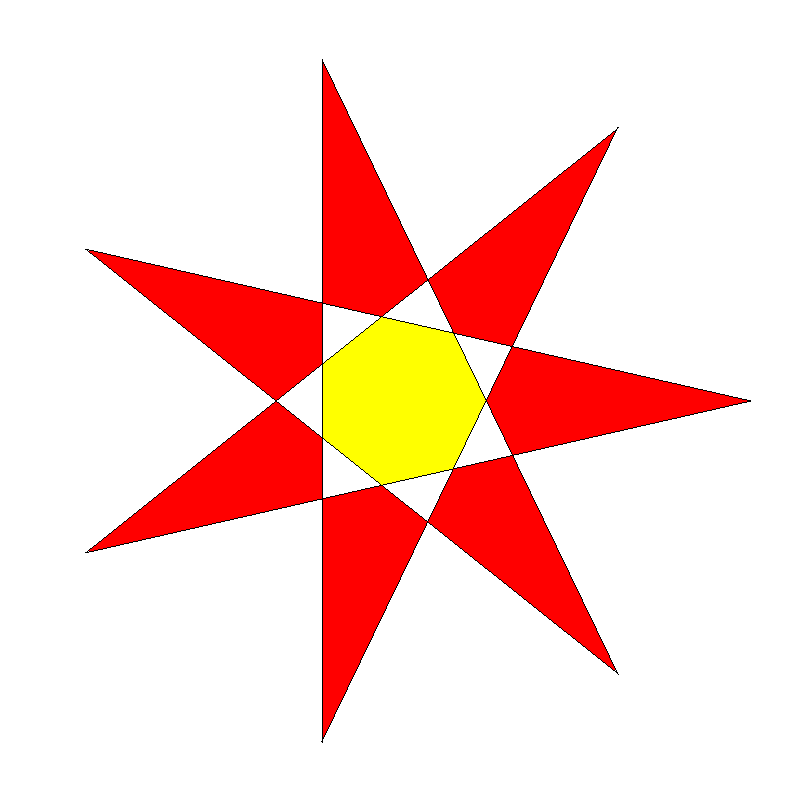
\includegraphics[width=0.9\textwidth]{data/m.7.3.png}}}
  \end{column}\hfill
  \begin{column}{0.45}
  \centerline{\fbox{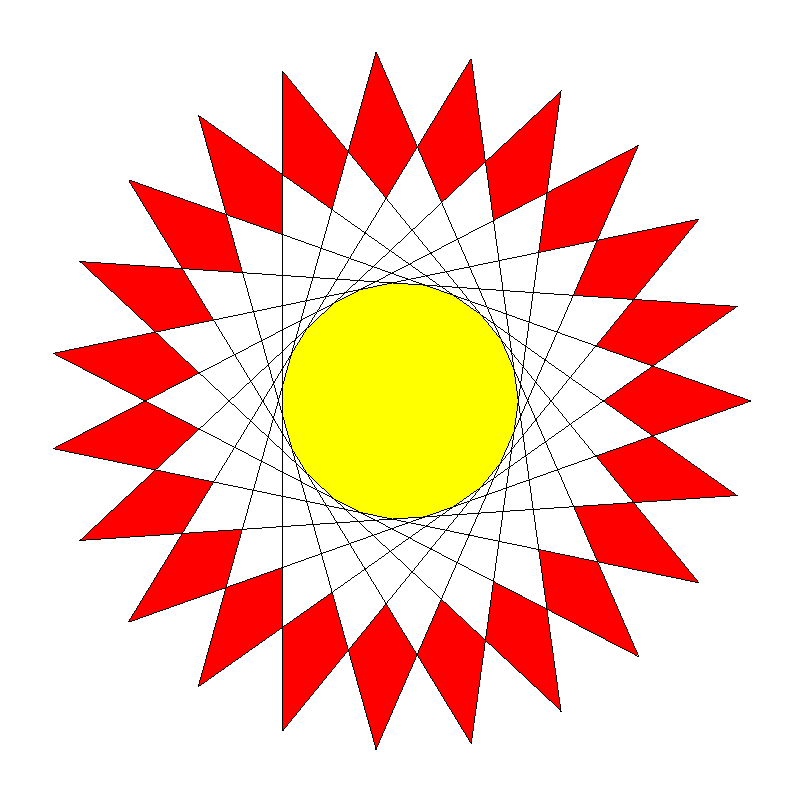
\includegraphics[width=0.9\textwidth]{data/m.23.9.png}}}
  \end{column}
  }
\end{uloha}

\def\ulohaTarget{None}
\vbox{
\begin{uloha}
  \indexItem{Alg}{korytnačia grafika}
  Korytnačia grafika pozostáva z postupnosti príkazov, každý na samostatnom riadku. 
  Príkazy sú takéto:
\def\tmp{\item \textcolor{magenta}}  
\begin{itemize}\itemsep=-1mm
    \tmp{\vb{i} {\em sirka vyska}} 
      (init) Toto je vždy prvý príkaz (a je v zozname iba
      raz). Nastaví rozmery obrázka. 
      \tmp{\vb{c} r g b} (color) Nastaví farbu na $\{r,g,b,255\}$.
    \tmp{\vb{u}} (pen up) Zdvihne pero -- nasledujúce posuny nekreslia.
    \tmp{\vb{d}} (pen down) Položí pero -- nasledujúce posuny kreslia.
    \tmp{\vb{f} x} (forward) Posunie sa dopredu o $x$.
    \tmp{\vb{l} a} (left) Otočí sa doľava o $a$ stupňov.
    \tmp{\vb{r} a} (right) Otočí sa doprava o $a$ stupňov.
    \tmp{\vb{s} meno} (save) Uloží obrázok a skončí.
\end{itemize}
Napíš program, ktorý načíta postupnosť príkazov korytnačej grafiky a vypíše
  postupnosť príkazov pre program z úlohy~\ref{uloha:editor}.
\end{uloha}
}
\def\ulohaTarget{File}


Na záver tejto časti skús rozšíriť korytnačiu grafiku o príkaz opakovania:

{\em
\def\tmp{\item \textcolor{magenta}}  
\begin{itemize}\itemsep=-1mm
      \tmp{\vb{R} cnt} (repeat) Blok príkazov po nasledujúci \vb{E} sa zopakuje
      {\em cnt} krát.
    \tmp{\vb{E}} (end) Koniec bloku opakovania.
\end{itemize}
}


Chceme, aby sa príkazy opakovania mohli vnárať, takže napr. program vľavo
urobí obrázok vpravo.

\begin{minipage}[t]{0.3\textwidth}\vspace{0pt}
\begin{Verbatim}
i 700 700
R 24
R 4
f 100
r 90
E
l 15
E
c 0 50 200
R 8
u
f 250
d
R 36
f 50
l 180
f 50
l 10
E
u
l 180
f 250
l 225
E
s logo.png
\end{Verbatim}
\end{minipage}
\hfill
\begin{minipage}[t]{0.7\textwidth}\vspace{0pt}{
  \setlength{\fboxsep}{0pt}
  \centerline{\fbox{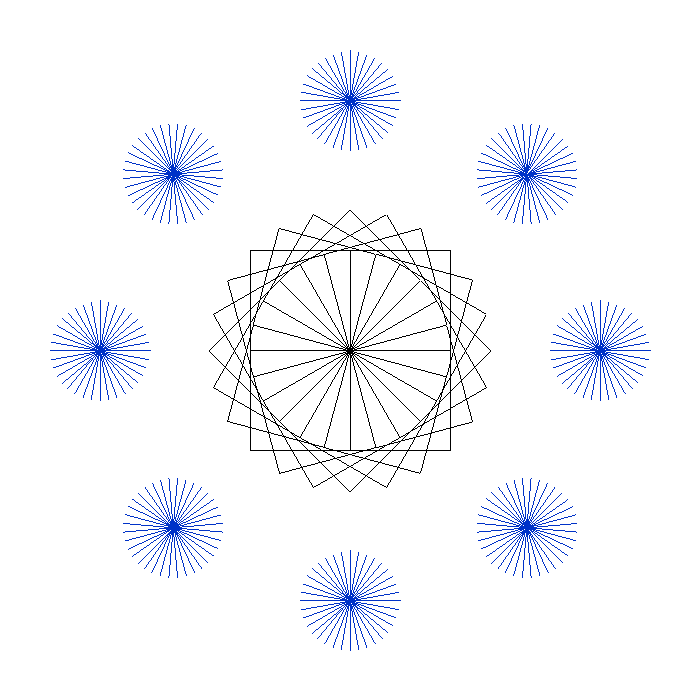
\includegraphics[width=\textwidth]{data/logo.png}}}
}
\end{minipage}


Na rozdiel od jednoduchšieho zadania bez cyklov, toto nemôžme riešiť tak, že 
príkazy čítame zo vstupu a priamo
vypisujeme príkazy pre kreslič, ale budeme si potrebovať všetky príkazy zapamätať.
Spravme si typ \vb{Prikaz}, v ktorom si budeme pamätať typ príkazu aj všetky
potrebné parametre (príkazy \vb{i} a \vb{s} ukladať nepotrebujeme, \vb{i} je vždy
na začiatku a \vb{s} je na konci: keď načítame zo vstupu \vb{s}, tak vygenerujeme
všetky zapamätané príkazy a skončíme). Okrem parametrov si v príkaze
\vb{R} budeme potrebovať pamätať terajší počet opakovaní pri vykonávaní 
a v príkaze \vb{E} si budeme potrebovať zapamätať pozíciu, kde je príslušný
príkaz \vb{R}. Celý typ by mohol vyzerať napr. takto:\\


\vbox{
\begin{lstlisting}[] 
struct Prikaz {
  char t;       // typ príkazu
  int r, g, b;  // pre príkaz 'c'
  double x;     // generický parameter pre príkazy 'l' 'r' 'f'
  int i, cnt;   // pre príkaz 'R'
  int addr;     // pre príkaz 'E'
};
\end{lstlisting}
}


Pri načítavaní vstupu si ukladáme príkazy do pamäte, pričom na príkazy \vb{R}
a \vb{E} použijeme zásobník ako v úlohe~\ref{uloha:zatvorky} na to, aby sme pre
každý príkaz \vb{E} našli zodpovedajúci príkaz \vb{R}. Začiatok programu z príkladu
by v poli vyzeral takto:


\centerline{
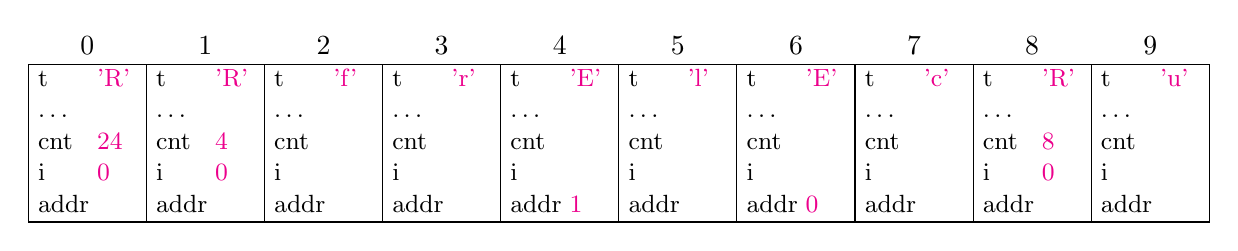
\begin{tikzpicture}[xscale=1.5,yscale=0.4]
    \def\cmd(#1)#2#3#4#5{
      \begin{scope}[shift={(#1,0)}]
        \draw (0,0) rectangle (1,5);
        \foreach \l [count = \i] in {addr,i,cnt,\ldots,t}{
          \node [anchor=south west] at (0,\i-1) {{\small\roboto \l}};
        }
        \foreach \v [count = \i] in {#5,#4,#3,{},'#2'}{
          \node [anchor=south west] at (0.5,\i-1) {{\small\roboto \textcolor{magenta}{\v}}};
        }
        \node [anchor=south] at (0.5,5) {$#1$};
      \end{scope}
      }

  \cmd(0)R{24}{0}{}
  \cmd(1)R{4}{0}{}
  \cmd(2)f{}{}{}
  \cmd(3)r{}{}{}
  \cmd(4)E{}{}{1}
  \cmd(5)l{}{}{}
  \cmd(6)E{}{}{0}
  \cmd(7)c{}{}{}
  \cmd(8)R{8}{0}{}
  \cmd(9)u{}{}{}
\end{tikzpicture}
}

Keď načítame celý program, začneme ho vyhodnocovať..
Budeme mať jednu globálnu premennú \vb{pc} (program counter),
v ktorej si budeme pamätať pozíciu práve vykonávaného príkazu. Bežné príkazy vždy 
spracujeme (tak, že vypíšeme na výstup príslušný príkaz pre kreslič) a zvýšime \vb{pc}.
V príkaze \vb{R} len zvýšime hodnotu \vb{i}. V príkaze \vb{E} sa pozrieme na hodnotu
\vb{i} v príslušnom \vb{addr}: ak sa rovná \vb{cnt}, vynulujeme ju a zvýšime \vb{pc},
ak nie, skočíme na príkaz \vb{R}. Ak sa pole príkazov volá \vb{prog} a
v premennej \vb{n} máme počet príkazov, vyhodnocovanie by vyzeralo zhruba takto:\\


\vbox{
\begin{lstlisting}[] 
void execute() {
  int pc = 0;
  while (pc < n) {
    if (prog[pc].t == 'R') {
      prog[pc].i++;
      pc++;
    } else if (prog[pc].t == 'E') {
      int jmp = prog[pc].addr;
      if (prog[jmp].i == prog[jmp].cnt) {
        prog[jmp].i = 0;
        pc++;
      } else {
        pc = jmp;
      }
    } else if .... 

    // tu sa spracujú ďalšie príkazy

  }
}


\end{lstlisting}
}


\begin{uloha}
  \label{uloha:logo}
  Naprogramuj korytnačiu grafiku s príkazmi cyklu.
\end{uloha}
